\question 某机器采用16位单字长指令,采用定长操作码,地址码为5位,现已定义60条二地址指令,那么单地址指令最多有(
)条
\par\twoch{\textcolor{red}{4}}{32}{128}{256}
\begin{solution}A。
首先可以计算出操作码字段的长度为16-5-5=6。因此,一共可以定义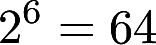
\includegraphics[width=0.56250in,height=0.16667in]{texmath/e1c5005Cdpi7B3507D25E63D64}条指令,既然二地址指令占了60条,且是定长操作码,故单地址指令最多可以有64-60=4条。如果此题将条件改为采用不定长操作码,答案又是什么?分析如下:
如果采用不定长(扩展)操作码,每条二地址指令可扩展为32条单地址指令,那么单地址指令最多有32×4=128条。
\end{solution}
\question 某计算机字长32位,CPU中有32个32位通用寄存器,采用单字长定长指令字格式,操作码占6位,其中还包含对寻址方式的指定。对于采用通用寄存器作为基址寄存器的RS型指令,则该指令的形式地址空间为
\par\twoch{\textcolor{red}{$2^16$}}{$2^21$}{$2^26$}{$2^32$}
\begin{solution}A。
基址寻址的RS型指令的一个操作数在寄存器中,另一个操作数在基址寻址的主存单元中,因为采用通用寄存器作为基址寄存器,所以必须在指令中明显指出基址寄存器是哪个通用寄存器,所以基址寄存器的编号占5位,
剩下的位数为32-6-5-5=16是位移量。则该指令的格式如下图所示:
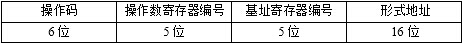
\includegraphics[width=3.33333in,height=0.31250in]{computerassets/5f6d4ab9dd73df215b670169449c0593.jpeg}~

故形式地址空间为2\^{}16,本题选A。 【扩展】
基址寄存器可采用隐式的和显示的两种。所谓隐式,是在计算机内专门设一个基址寄存器BR,使用时用户不必明显指出该基址寄存器,只需要指令的寻址特征位反映出基址寻址即可。显式是在一组通用寄存器里,由
用户明确指出哪个寄存器用做基址寄存器,存放基地址。本题属于显式的情况。
\end{solution}
\question 某计算机有16个通用寄存器,采用32位定长指令字,操作码字段(含寻址方式位)为8位,Store指令的源操作数和目的操作数分别采用寄存器直接寻址和基址寻址方式。若基址寄存器可使用任一通用寄存器,且偏移量用补码表示,则Store指令中偏移量的取值范围是(
)
\par\twoch{\textcolor{red}{-32768~+32767}}{-32767~+32768}{-65536~+65535}{-65535~+65536}
\begin{solution}本题考察的是指令的寻址方式,这题可以采用排除法直接排出B、D选项,因为无论偏移量占多少位,由于偏移量是用补码表示的,它比原码表示的数要多出一个,而且多出的这一个正是补码表示的最小值,所以要么是-32768,要么是-65536。题目中是32位指令,操作码8位(已经包含了寻址方式)源操作数采用寄存器直接寻址,故可以采用4位来标记使用哪个寄存器,目的操作数采用基址寻址,由于题目告诉可以使用任一通用寄存器,故需要采用4位来标记,所以偏移量所占位数=32-8-4-4=16位,故偏移量的取值范围是-32768\textasciitilde{}+32768(含1位符号位)。
【总结】在考场上有时候即使我们不能一步就算出结果,或者题目复杂的时候,可以抓住问题的一些细节来排出某些选项,这对我们分析余下的选项也是很有帮助的,另外指令的各种寻址方式也一定要掌握,这里的偏移量是对形式地址的另外一种表示。
\end{solution}
